\documentclass{ReportTemplate}
\usepackage{titlesec}
\usepackage[francais]{babel}
\usepackage[T1]{fontenc}
\title{CSEL}
\author{Macherel Rémy}
\date{\today}
\subtitle{Rapports des TP}
\subsubtitle{Git du projet : \href{https://github.com/Mathistis/csel-workspace}{https://github.com/Mathistis/csel-workspace}}
\location{Fribourg,}
\contact{remy.macherel@master.hes-so.ch}
\version{1.0}
\titlespacing*{\chapter}{0pt}{-60pt}{20pt}
\begin{document}

\maketitlepage

\newpage

\maketableofcontent

\medskip

\titleformat{\chapter}[display]
    {\Huge\bfseries}
    {}
    {0pt}
    {\thechapter.\ }
    

\chapter{Introduction}
Ce rapport décrit l'architecture ainsi que le développement et les
fonctionnalités du mini-projet réalisé lors du cours \textit{MA-CSEL} suivi lors
du semestre de printemps 2022 du master MSE. Ce projet consiste à mettre en
pratique les notions vues dans le cours par l'intermédiaire de l'implémentation
d'un gestionnaire de ventilateur pour le processeur de la cible. Notre cible
n'ayant pas de réel ventilateur, son fonctionnement sera simulé par le
clignotement d'une LED symbolisant la fréquence de celui-ci ainsi qu'un écran
OLED affichant quelques valeurs importantes.\newline
Le but du travail est donc de concevoir une application permettant de simuler la
gestion de la vitesse de rotation d'un ventilateur en fonction de la température
du processeur. Les fonctionnalités suivantes seront donc implémentées:
\begin{itemize}
    \item Supervision de la température du processeur et la gestion de la
    vitesse de clignotement de la LED à l'aide d'un module noyau.
    \item Un daemon en espace utilisateur qui offrira des services pour une
    gestion manuelle et prendra en compte la gestion des appuis sur les boutons
    afin d'augmenter la vitesse de rotation, de la diminuer et de passer du mode
    manuel à automatique.\newline
    Ce daemon pourra également, à l'aide d'une interface IPC, communiquer avec
    une application de type \textit{CLI} pour la gestion du clignotement et du
    mode.
    \item Une application \textit{CLI} pour piloter le système via l'interface IPC.
\end{itemize}

\chapter{Architecture logicielle}
\begin{figure}[H]
    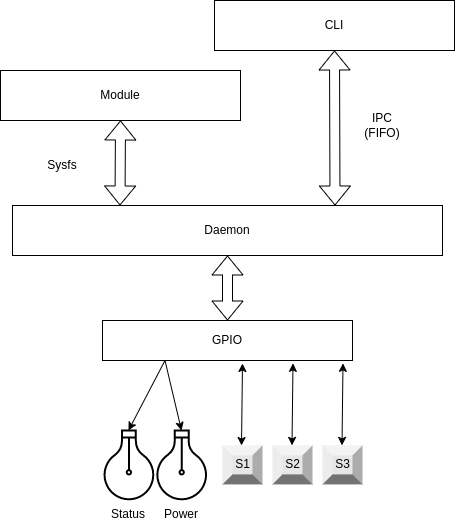
\includegraphics[width= \textwidth]{imageSources/Diagramme_Fonctions.drawio.png}
    \caption{Diagramme de principe de l'application}
    \label{fig:functionDiagram}
\end{figure}
\chapter{Conception du module}
Ce chapitre traite du développement du module noyau permettant de surveiller la
température du processeur ainsi que la gestion du clignotement de la LED status.
Ce module utilise le sysfs afin de gérer les deux modes de fonctionnement
(manuel/automatique) et la fréquence de clignotement de la led Status. Selon les
spécifications, les différentes fréquences de clignotement de la led sont :
\begin{figure}[H]
    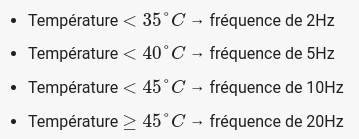
\includegraphics[width= \textwidth]{imageSources/Led_Frequencies.png}
    \caption{Fréquences pour la led en mode automatique}
    \label{fig:ledFrequencies}
\end{figure}
Dans le module, nous avons séparé les codes en deux parties, un fichier
\textit{controller.c} (avec son .h dédié) qui représente une bibliothèque
permettant la gestion des modes du programme. Ce controller permet d'initialiser
les différents éléments utilisés dans le module (comme gpio, capteur de
température, timers, etc.), il sert en quelque sorte d'interface de gestion des
éléments du module noyau.\newline
Le deuxième fichier \textit{gpio.c} (également accompagné de son .h) permet quand à lui la gestion
des gpio ainsi que leur initialisation.\newline
Un autre code présent dans l'utilisation du module est le
\textit{temp\_controller}, celui-ci permet à l'aide de la bibliothèque
\textit{linux/thermal.h} de récupérer la température actuelle du
processeur.\newline
Toutes ces fonctions sont alors utilisées (via le controller) dans le fichier
\textit{skeleton.c} dans celui-ci se trouvent les différentes méthodes
permettant d'actualiser via le sysfs les états des leds.\newline
Ce module va également créer et initialiser dans le sysfs les fichiers
nécessaires à la transmission de nos informations.
\begin{figure}[H]
    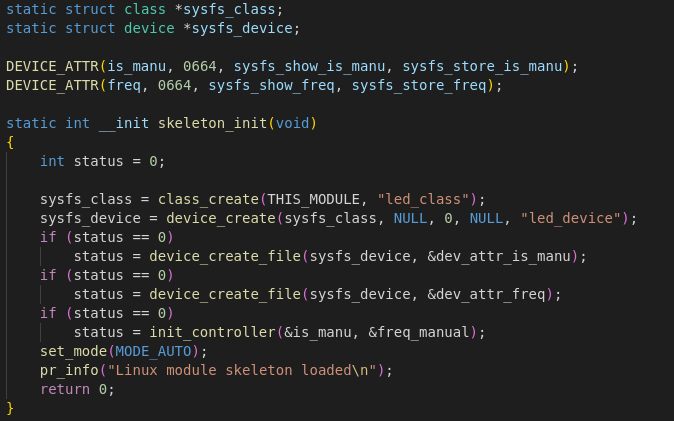
\includegraphics[width= \textwidth]{imageSources/sysfs_init.png}
    \caption{Création des fichiers nécessaires dans le sysfs}
    \label{fig:sysfsInit}
\end{figure}
\chapter{Conception du daemon}
Ce chapitre traite du développement du deamon offrant les services permettant la
gestion de la fréquence ainsi que le choix du mode.

\end{document}


